\documentclass{article}

\usepackage[final]{style}
\usepackage[utf8]{inputenc} % allow utf-8 input
\usepackage[T1]{fontenc}    % use 8-bit T1 fonts
\usepackage{hyperref}       % hyperlinks
\usepackage{url}            % simple URL typesetting
\usepackage{booktabs}       % professional-quality tables
\usepackage{amsfonts}       % blackboard math symbols
\usepackage{nicefrac}       % compact symbols for 1/2, etc.
\usepackage{microtype}      % microtypography
\usepackage{verbatim}
\usepackage{graphicx}       % for figures
\usepackage{amsmath}
\usepackage{algorithm}
\usepackage{algpseudocode}
\makeatletter
\def\BState{\State\hskip-\ALG@thistlm}
\makeatother

\title{Lecture \#9: Image Resizing and Segmentation}

\author{
  Mason Swofford, Rachel Gardner, Yue Zhang, Shawn Fenerin \\
  Department of Computer Science\\
  Stanford University\\
  Stanford, CA 94305 \\
  \texttt{\{mswoff, rachel0, yzhang16, sfenerin\}@cs.stanford.edu} \\
}

\begin{document}

\maketitle

\section{Introduction}
The devices used for displaying images and videos are of different sizes and shapes. The optimal image/video viewing configuration, therefore, varies across devices and screen sizes. For this reason, image resizing is of great importance in computer vision. The intuitive idea is to rescale or crop the original image to fit the new device, but that often causes artifacts or even loss of important content in images. This lecture discussed the techniques used for resizing images while preserving important content and limiting the artifacts.
\subsection{Problem Statement}
Input an image of size $n\times m$ and return an image of desired size $n'\times m'$ which will be a good representative of original image. The expectations are:
\begin{enumerate}
\item The new image should adhere to device geometric constraints.
\item The new image should preserve the important content and structures.
\item The new image should have limited artifacts.
\end{enumerate}
\subsection{Importance Measures}
\begin{enumerate}
\item A function, $S: p \rightarrow [0,1]$, is used to determine which parts in an image are important; then, different operators can be used to resize the image. One solution is to use an optimal cropping window to extract the most important contents, but this may result in the loss of important contents.
\begin{figure}[H]
\centering
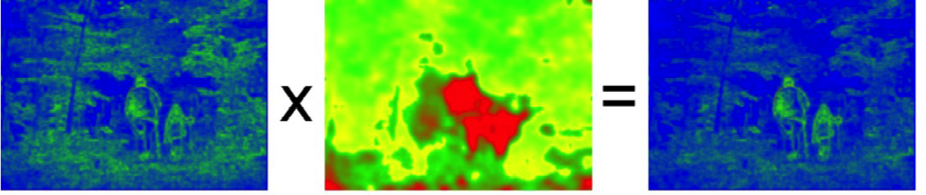
\includegraphics[width=8cm]{Function.png}
\caption{Importance Measurement by function method. Source: Lecture 7-11.}
\end{figure}
\item There are also more sophisticated techniques for measuring the image regions with higher degree of important content; they include, but are not limited to, attention models, eye tracking (gaze studies), and face detectors.
\begin{figure}[H]
\centering
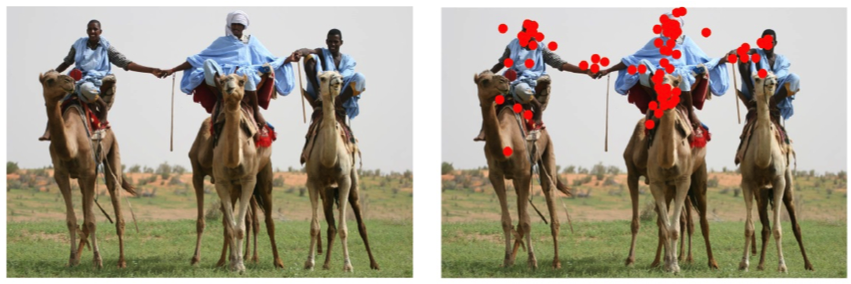
\includegraphics[width=8cm]{Tracking.png}
\caption{Importance Measurement by more sophisticated methods such as eye tracking. Source: Lecture 7-11, \cite{judd2009learning}}
\end{figure}
\end{enumerate}

% Lecture 7 - 20 to 40
% Yue
% Gustavo 40 to 60
\section{Seam Carving}
\subsection{Basic Idea}
The human vision is more sensitive to the edges in an images. Thus, a simple but effective solution is to remove contents from smoother areas and preserve the more informative image regions that contain edges; this is achieved using a gradient-based energy function, defined as:
$$
E(I) = |\frac{\partial}{\partial x}I| + |\frac{\partial}{\partial y}I|
$$
Unimportant contents are, therefore, pixels with smaller values of energy function.
\subsection{Pixel Removal}
There exist different approaches for removing the unimportant pixels, and each can lead to different visual results. The figure below demonstrates three examples of such approaches; the first two (i.e., optimal least-energy pixel and row removal) are observed to negatively affect the image quality. The last one (i.e., least-energy column removal), on the other hand, works significantly better, but it still causes plenty of artifacts in the new image. An alternative solution is presented in the next section.
\begin{enumerate}
\item Removing all pixels with less energy.
\item Removing the rows of pixels with the least energy.
\item Removing the columns of pixels with the least energy.
\end{enumerate}
\begin{figure}[H]
\centering
\hspace*{1.2cm}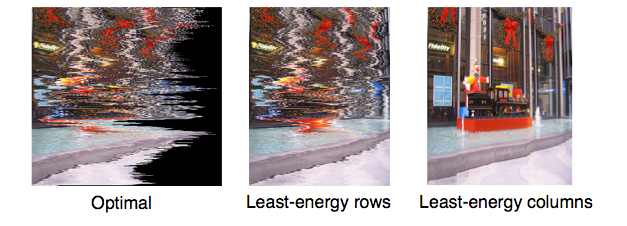
\includegraphics[width=8cm]{Pixel_Removal.png}
\caption{The effects of different pixel removal methods on the image quality. Source: Lecture 7-18}
\end{figure}
\subsection{A Seam}
\begin{enumerate}
\item A seam is defined as a connected path of pixels from top to bottom (or left to right). For top-to-bottom pixel, we shall pick exactly one pixel from each row. The mathematical definition is
$$
s^x = \{s_i^x\}_{i=1}^n = \{x(i),i\}_{i=1}^n, s.t. \forall i, |x(i) - x(i - 1)| \leq 1
$$
$$
s^y = \{s_j^y\}_{j=1}^m = \{j,y(j)\}_{j=1}^m, s.t. \forall j, |y(j) - y(j - 1)| \leq 1
$$
\item The optimal seam is the seam which minimizes the energy function, based on pixel gradients.
$$
s^{*} = argmin_s E(s), \quad \textrm{where} \quad E(I) = |\frac{\partial}{\partial x}I| + |\frac{\partial}{\partial y}I|
$$
\begin{figure}[H]
\centering
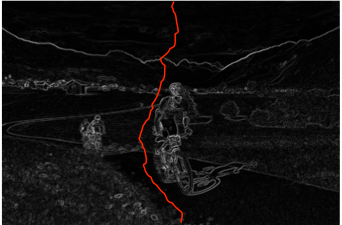
\includegraphics[width=8cm]{Optimal_Seam.png}
\caption{The red line indicates the location of the optimal seam with the least energy. Source: Lecture 7-22}
\end{figure}
\item The recursion relation can be used to find the optimal seam. If $M(i,j)$ is defined as the minimal energy cost of a seam going through pixel $(i,j)$, the recursion relation is
$$
M(i,j) = E(i,j) + min(M(i-1,j-1), M(i-1,j), M(i-1,j+1))
$$
This problem can be solved efficiently by using dynamic programming in $O(snm)$, $s=3$ in the original algorithm.
Given the energy function value as
\begin{figure}[H]
\centering
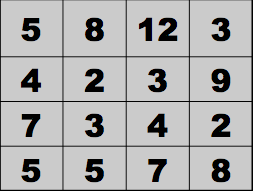
\includegraphics[width=4cm]{energy.png}
\caption{An example of energy function used in seam carving algorithm. Source: Lecture 7-24}
\end{figure}
The recursion relation gives
\begin{figure}[H]
\centering
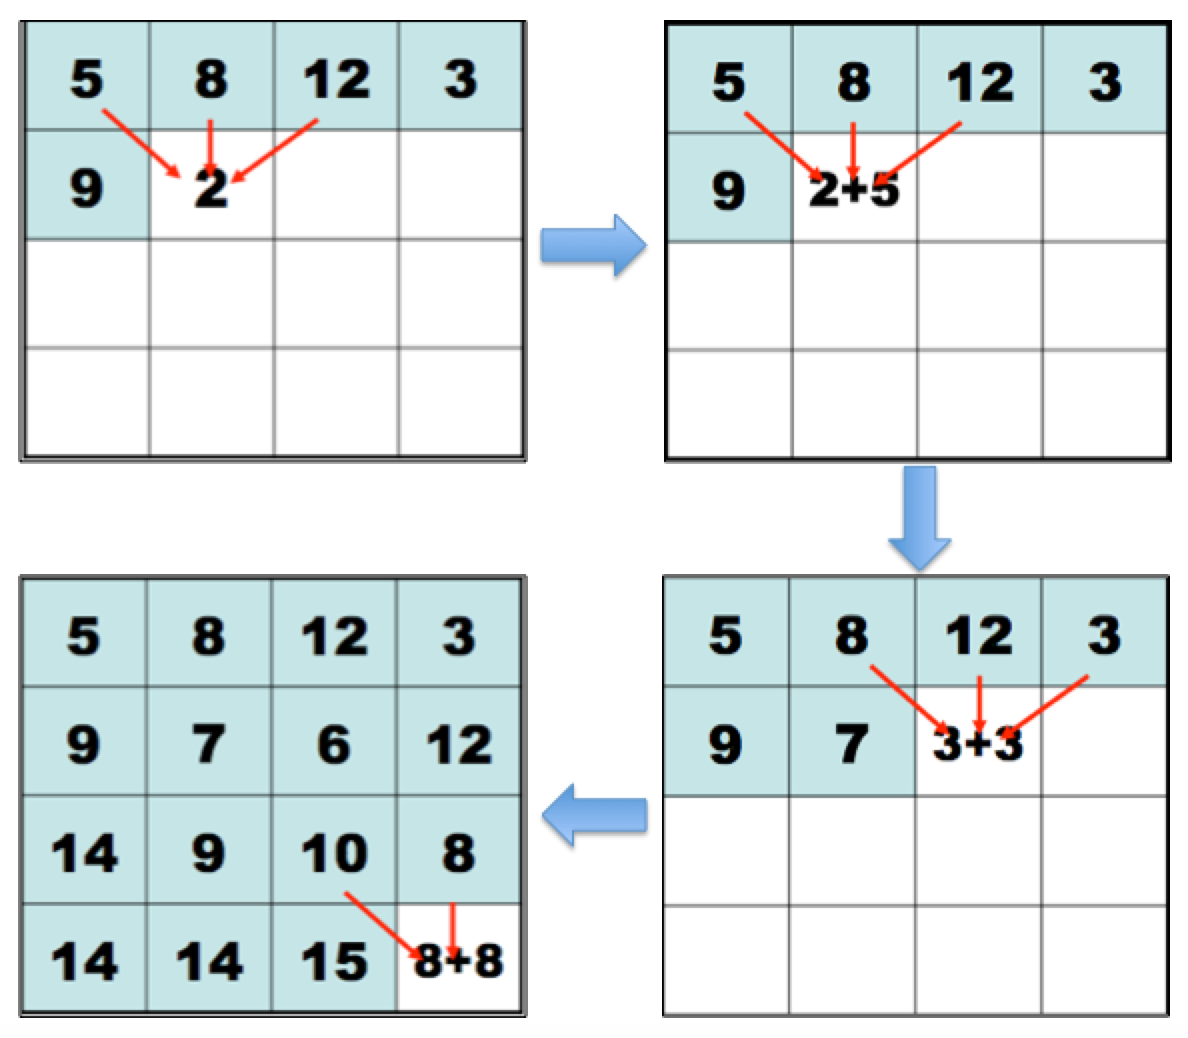
\includegraphics[width=8cm]{findseam1.png}
\caption{The process of using relation recursion for computing the seam cost. Source: Lecture 7-(24-27)}
\end{figure}
\item To search for the optimal seam, backtracking method is introduced. It starts from the pixel at the bottom with the lowest energy function, and it then goes up toward the top of the image (i.e., first image row).
\end{enumerate}
\begin{figure}[H]
\centering
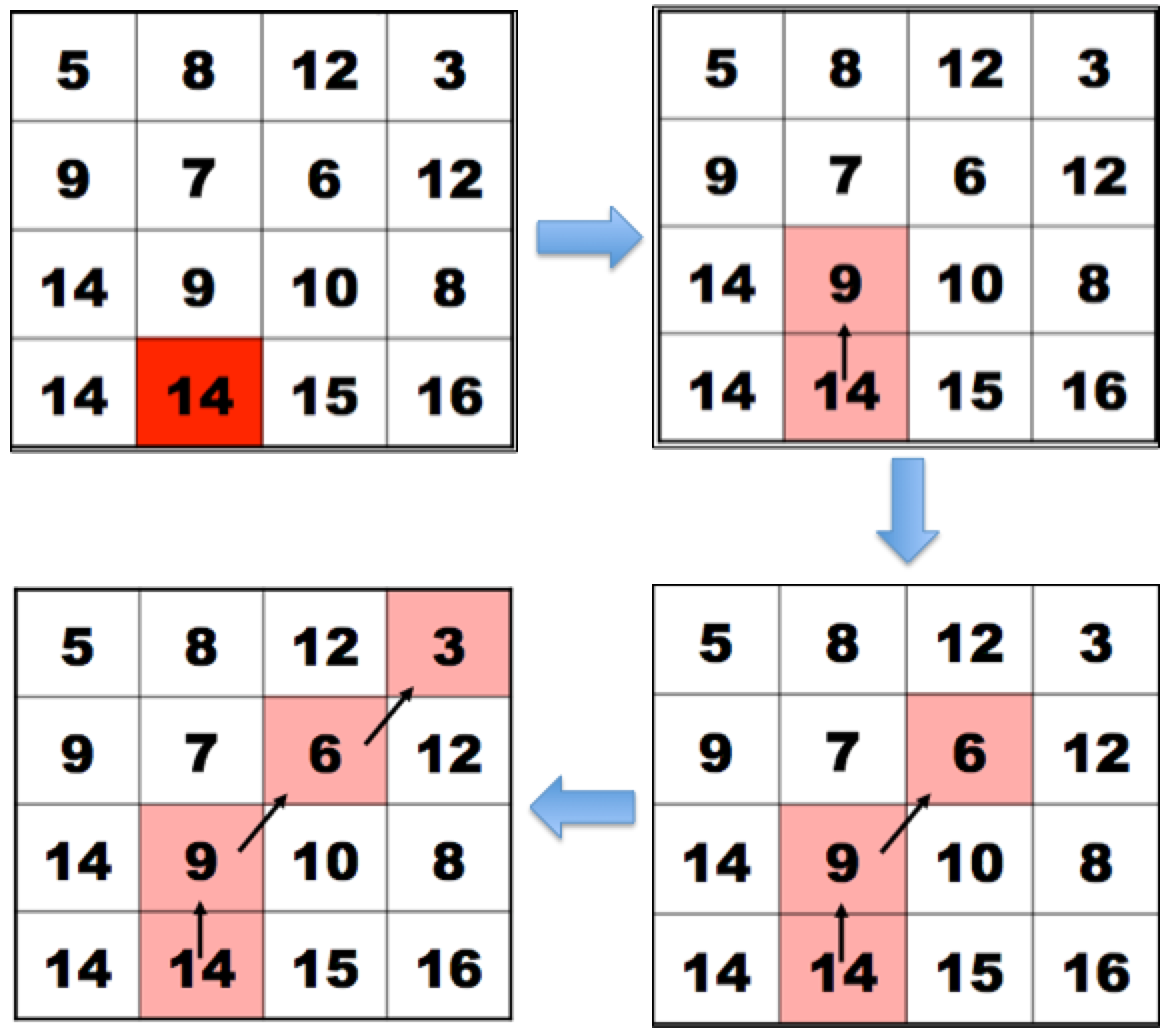
\includegraphics[width=8cm]{backtrack.png}
\caption{Using backtrack to find the optimal seam. Source: Lecture 7-(28-31)}
\end{figure}
\subsection{Seam Carving Algorithms}
This algorithm runs $O((n-n')mn)$. In each loop, each update of $E$, $s$ and $im$ takes $O(mn)$. For vertical resizing, the image could be transposed so that the same algorithm can be used.
\begin{algorithm}
\caption{Seam-Carving}\label{euclid}
\begin{algorithmic}[1]
\State $im \gets \textit{original image of size m $\times$ n}$
\State $n' \gets \textit{desired image size n'}$
\State
\BState \emph{Do (n-n') times}:
\State \hspace{0.5cm} $E \gets \textit{Compute energy map on im}$
\State \hspace{0.5cm} $s \gets \textit{Find optimal seam in E}$
\State \hspace{0.5cm} $im \gets \textit{Remove s from im}$
\State
\BState \emph{return im}
\end{algorithmic}
\end{algorithm}


The average energy of images increase given that the seam carving algorithm removes low energy pixels. The described seam carving algorithm can be used to modify aspect ratio, to achieve object removal, and to perform image resizing. The process is the same if an image is flipped. When resizing, both horizontal and vertical seams need to be removed. One can solve the order of adding and removing seams in both directions by dynamic programming. Specifically, the recurrence relation is: $T(r,c)=min(T(r-1,c)+E(s^x(I_{n-r-1\times m-c})),T(r,c-1)+E(s^y(I_{n-r\times m-c-1})))$ for more information refer to the SIGGRAPH paper on seam carving \cite{siggraphseamcarving}.

\begin{center}
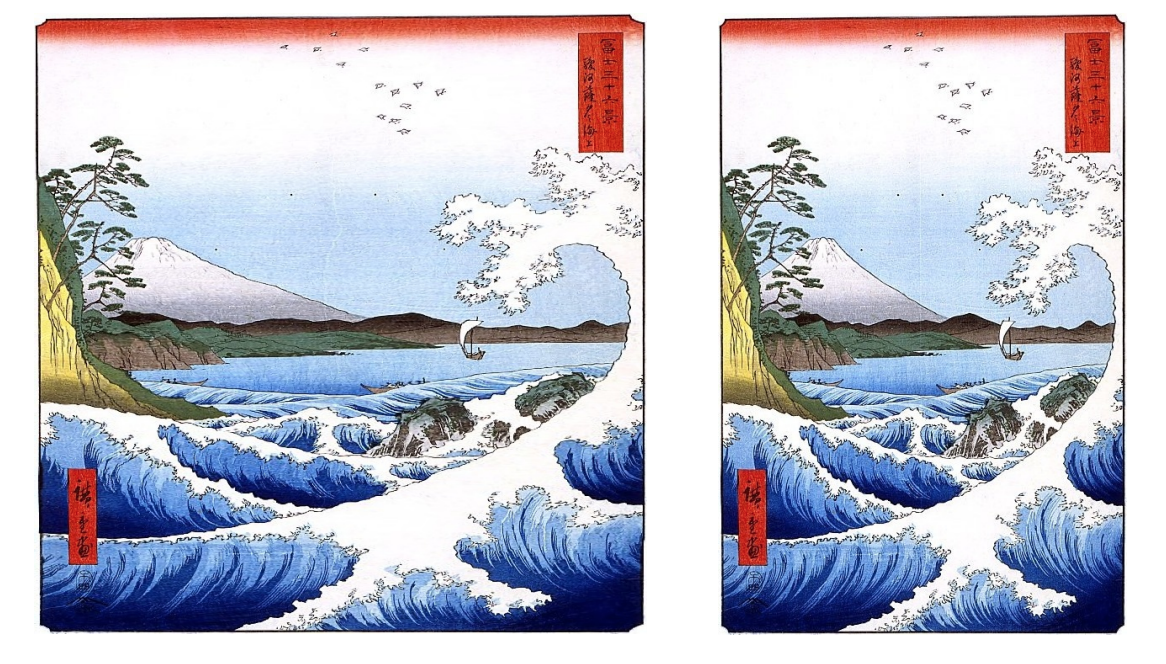
\includegraphics[width=8cm]{content_aware_resizing.png} \\
Figure 8: The Sea off Satta, Hiroshige woodblock print (Public Domain)
\end{center}

% Lecture 7 - 60 to [end]
% Rachel
\section{Advanced Seam Carving}
\subsection{Image Expansion}
A similar approach can be employed to increase the size of images. By expanding the least important areas of the image (as indicated by our seams), the image dimensions can be increased without impacting the main content. A naive approach is to iteratively find and duplicate the lowest energy seam. However, this provides us results as depicted below:

\begin{center}
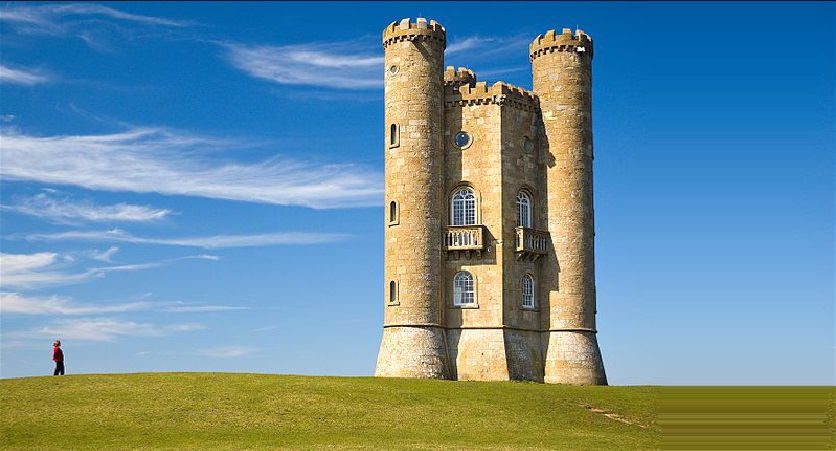
\includegraphics[width=8cm]{Naive_Castle_Resizing.jpg} \\
Figure 9: Duplicating the least-energy seam is not a good strategy for image expansion \cite{castle}
\end{center}
On the right side of the image (Figure 9), one seam has been duplicated repeatedly. This is the program retrieves the same (least-energy) seam repeatedly. A more effective implementation is to find the first $k$ seams at once and duplicate each:

\begin{center}
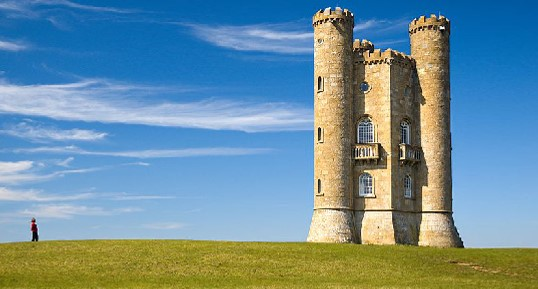
\includegraphics[width=8cm]{Smart_Resizing.jpg} \\
Figure 10: A more effective image expansion strategy using the first $k$ low-energy seams \cite{castle2}
\end{center}
As observed above, the second image expansion strategy significantly improves the quality of resized image. Note, however, that this method can only enlarge the image by a factor of 2 (since there simply aren't enough seams to duplicate). For very dramatic enlargements, you can instead iteratively enlarge by 1.4-1.5x.

\subsection{Multi-Size Image Representation}
While we've seen that image resizing can be very effective, it is still very computationally intensive. In practice, images are stored alongside a representation of their seams to forgo seam re-calculation of the seams and streamline image resizing on devices. These seam representations are the same dimensions as the image, but instead of pixel intensities, they have numbered paths ordering seams based on their energy values (ranging from least-energy to highest-energy). In order to calculate these seams in the pre-processing step, the image energy must be recalculated after each seam removal (this is because of the changes in the cost function). See below for an example of such a representation:
\begin{center}
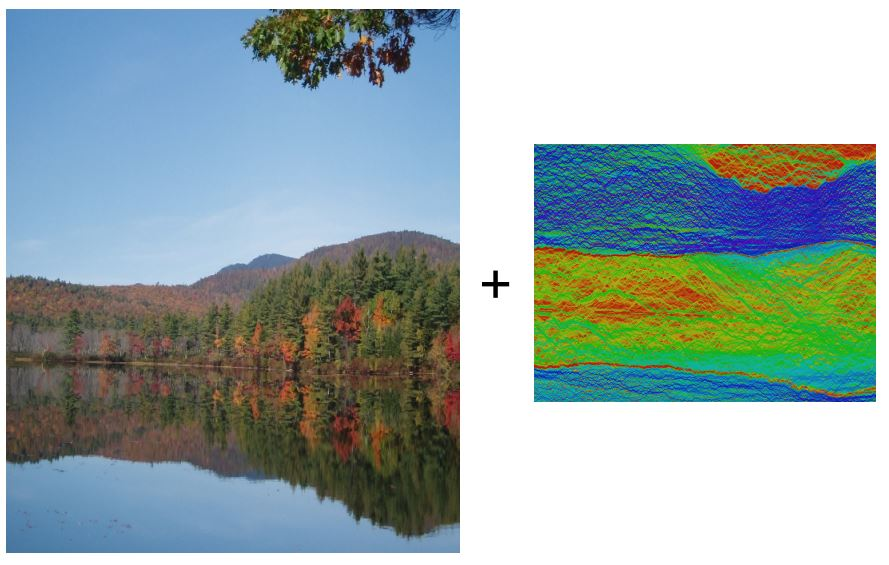
\includegraphics[width=8cm]{resizing_representation.JPG} \\
Figure 11: Examples of pre-computed seams used for fast image resizing on devices \cite{siggraphseamcarving}.
\end{center}
Given this representation, a program seeking to remove $k$ seams from the original image can remove the pixels corresponding to those labeled 1 through $k$ in the seam image (at right).
\subsection{Object Removal}
By allowing users to specify which areas of the image to give high or low energy, we can use seam carving to specifically preserve or remove certain objects. The algorithm chooses seams specifically so that they pass through the given object (in green below).

\begin{center}
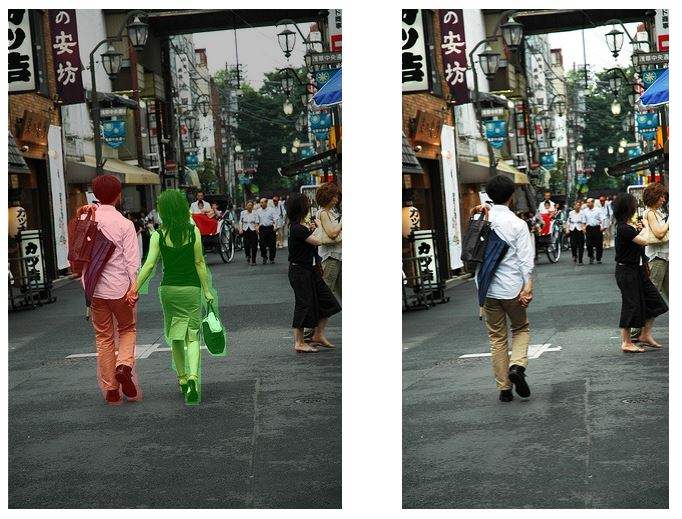
\includegraphics[width=8cm]{object_removal.JPG} \\
Figure 12: The seam carving algorithm can be used for object removal by assigning low energy values to part of the image \cite{siggraphseamcarving}.
\end{center}

%Shawn Fenerin
\subsection{Limitations}
Seam carving is an effective method for image resizing. However, there are limitations: 1) the primary limitation is the lower and upper limit to effectiveness as the size of the image is drastically changed; 2) the failure in recognizing important features in the context of an object that can be low energy. Let us consider the image below.
\begin{center}
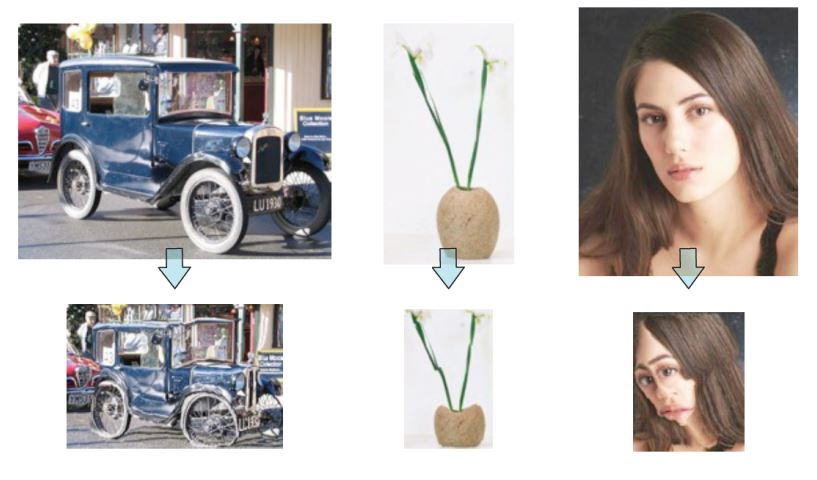
\includegraphics[width=8cm]{seam_carving_limitations.JPG} \\
Figure 13: The limitations of seam carving; source: CS131 Lecture 7, slide 71
\end{center}

While the flat and smooth image regions (i.e., with low gradients) are important to the image, they are removed; for example, this includes the woman's cheeks and forehead. While these regions are low in energy, they are important features to human perception and should be preserved. To address such limitations, the energy function can be modified to consider additional information. For example, a face detector can be used to identify important contents (i.e., human faces) or other constraints can be applied by the users.

\begin{center}
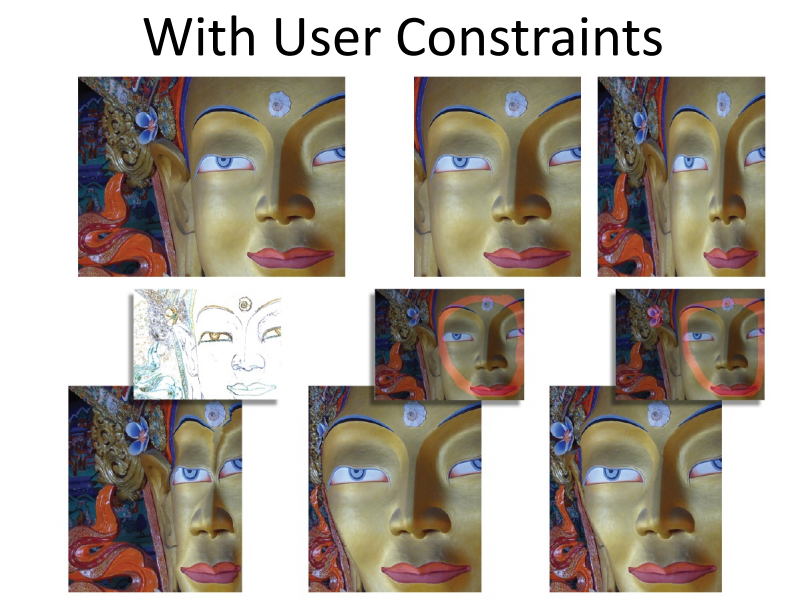
\includegraphics[width=8cm]{user_constraints.PNG} \\
Figure 14: Seam Carving	for	Content-Aware Image	Resizing \cite{avidan2007seam}.
\end{center}
% * <sfenerin@stanford.com> 2017-10-31T02:00:41.390Z:
%
% ^.

\subsection{Forward Energy}
When we carve seams, we are removing the lowest energy pixels and preserving the highest energy pixels. Hence, the average image energy is increased and can lead to artifacts and jagged edges. One way to avoid this issue is to instead focus on removing seams that insert the least energy into the image. This approach is known as the forward energy; our original accumulated cost matrix is modified by adding the forward energy from corresponding new neighbors as seen in the image below. The originally introduced method is referred to as "backward" energy.

\begin{center}
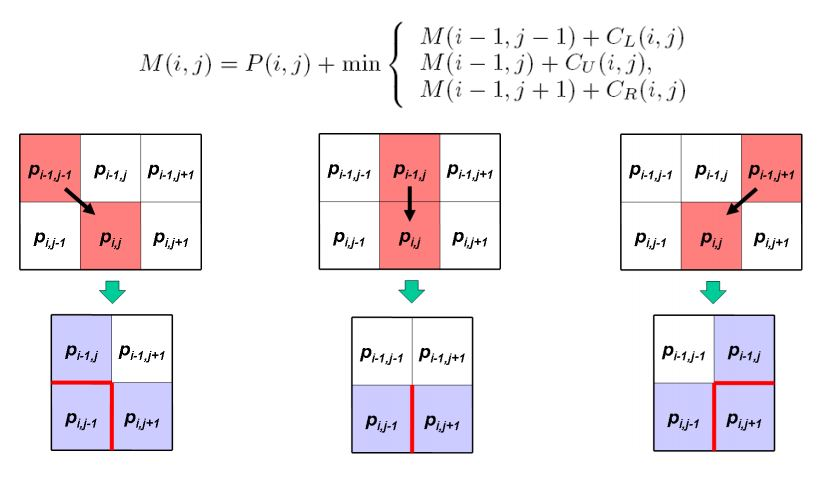
\includegraphics[width=8cm]{forward_energy_calculation.JPG} \\
Figure 15: The forward energy calculations; source: Lecture 7-71
\end{center}

Figure 15 gives us 3 cases of removing seam containing pixel $p(i,j)$. Calculating the three possible vertical seam step costs for pixel $p(i,j)$ using forward energy. After removing the seam, new neighbors (in gray) and new pixel edges (in red) are created. In each case the cost is defined by the forward difference in the newly created pixel edges. This is because at each step, we search for the seam whose removal inserts the minimal amount of energy into the image. These are seams that are not necessarily minimal in their energy, but will leave less artifacts in the resulting image, after removal. Note that the new edges created in row $i-1$ were accounted for in the cost of the previous row pixel. 

Thus we have 
$$C_L(i,j) = \|I(i,j+1) - I(i,j-1)\| + \|I(i-1,j) + I(i, j-1) \|$$

$$C_R(i,j) = \|I(i,j+1) - I(i,j-1)\| + \|I(i-1,j) + I(i, j+1) \|$$

$$C_U(i,j) = \|I(i,j+1) - I(i,j-1)\|$$.

The figure below compares the performance of backward and forward computations for image resizing. The traditional "backward" energy approach resulted in jagged edges appearing along the handle of the wrench and the stem of the plant. The "forward" energy approach, on the other hand, minimizes the added energy, and the smoothness of the edges is maintained.

\begin{center}
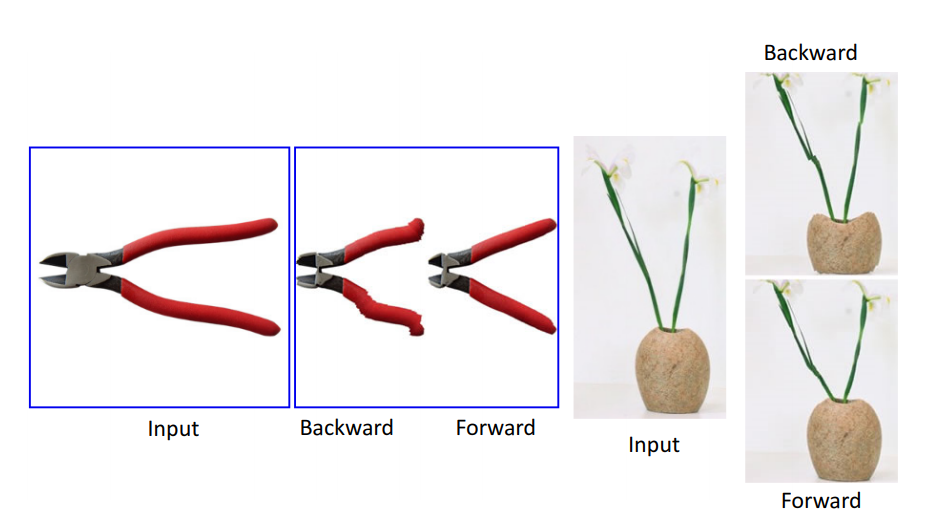
\includegraphics[width=8cm]{forward_energy.PNG} \\
Figure 16: Forward energy approach for content-aware image resizing \cite{avidan2007seam}.
\end{center}

\subsection{Seam-Carving in Videos}
While the powerful capabilities of seam carving is explored, the question remains as to how it can be applied to videos. This algorithm faces challenges with respect to video resizing. Videos are significantly more difficult to resize. We face two primary issues.

First, let us consider a one-minute window of a film recorded at 30fps. In that duration, we have 1800 frames. If our seam carving algorithm takes a full minute to process an image, it would take us 30 hours to completely process the video.

The second issue is with temporal coherency. One can consider the intuitive and naive approach of seam carving to process each frame independently. However, this does not necessarily preserve the important content with respect to the relation of consecutive frames. Since the human eye is particularly sensitive to movement, the failure to consider the context across images can create a poor looking video with noticeable distortion from frame to frame. There is no coherency to changes across frames. A more effective approach is to consider the video as a three dimensional space where each vertical plane is an image from the video. The lowest energy 2D seam can be calculated throughout the entire video's length. This produces much better results, but it still faces limitations.
\begin{center}
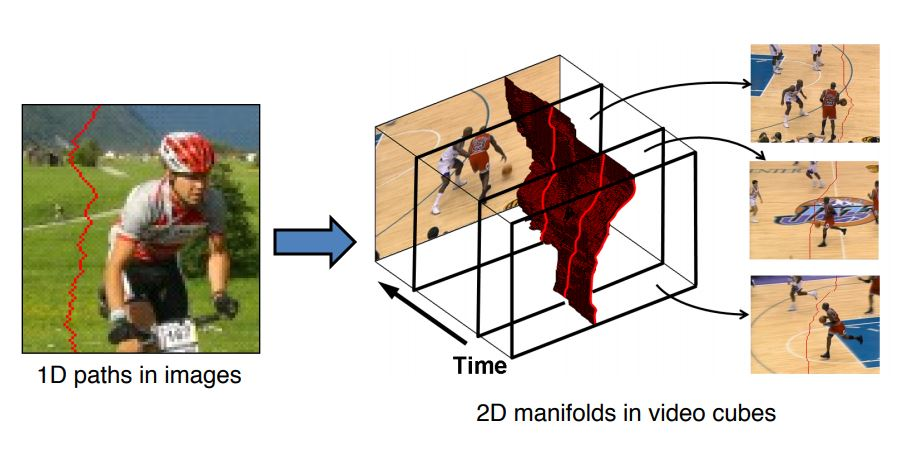
\includegraphics[width=8cm]{video_retargeting.JPG} \\
Figure 17: Improved Seam Carving for Video Retargeting \cite{rubinstein2008improved}.
\end{center}

This 3D representation gives us the same capabilities as 2D Seam-Carving such as object removal and frame resizing.
% Lecture 12 - 1 to 20
% Mason
\section{Segmentation}
In computer vision, we are often interested to identify groups of pixels that go together. We call this problem image segmentation. Humans perform image segmentation by intuition. For instance, two people looking at the same optical illusion might see different things, all depending on how their brain segments the images. In the image below, you might see zebras, or you might see a lion.
\begin{center}
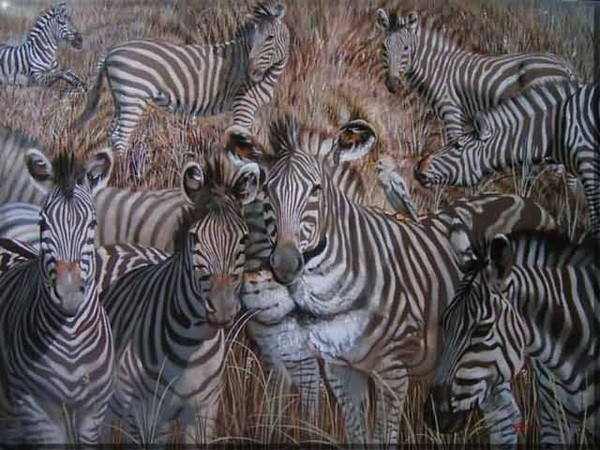
\includegraphics[width=8cm]{lion.jpg} \\
Figure 18: Optical illusions regarding the problem of image segmentation \cite{illusion}.
\end{center}

One of the motivations behind image segmentation is the separation of an image into coherent objects. Here are two examples of this type of segmentation:

\begin{center}
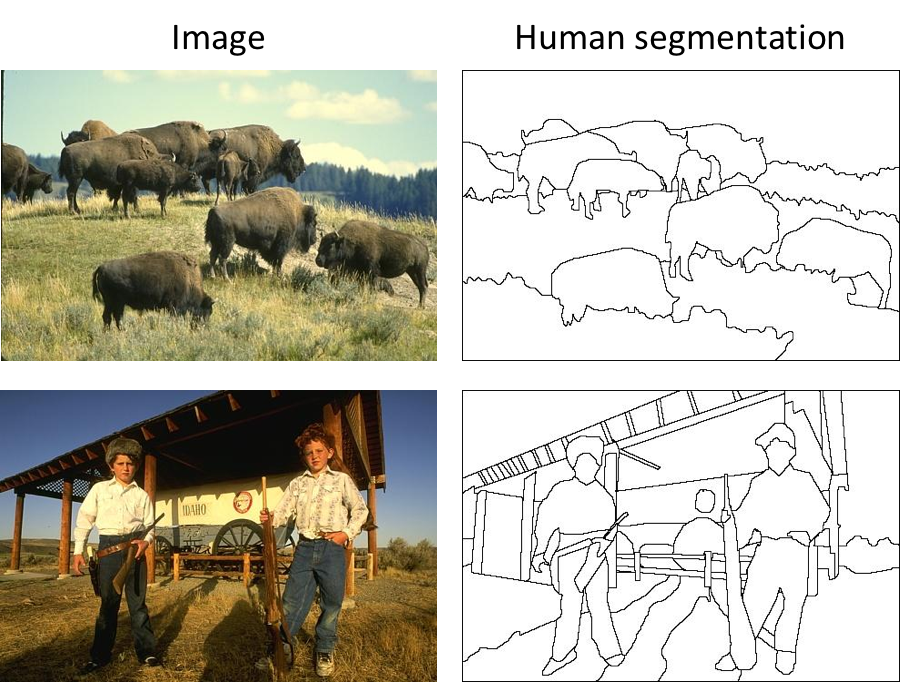
\includegraphics[width=8cm]{objects.png} \\
Figure 19:  Human segmentation of example images; source: Svetlana Lazebnik
\end{center}

We might also want to segment an image into many groups based off nearby pixels being similar. We call these groups "superpixels." Superpixels allow us to treat many individual pixels as one cluster, and therefore enable faster computations. Here is an example of an image segmented by superpixels:

\begin{center}
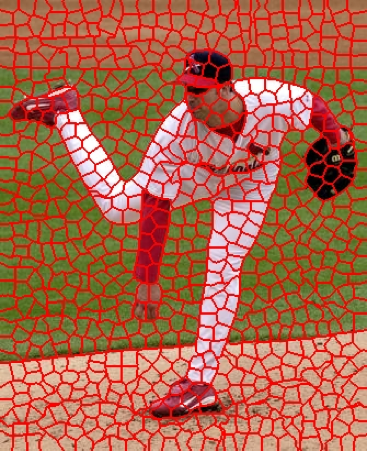
\includegraphics[width=8cm]{superpixels.png} \\
Figure 20: The superpixels allow faster computations by clustering pixels \cite{ren2003learning}.
\end{center}

Superpixel segmentation and other forms of segmentation can help in feature support. We can treat the groups of pixels as one feature and garner information about the image from them.Image segmentation is also beneficial for some common photo effects such as background removal. If we can properly segment an image, we will be able to only keep the groups we want and remove the others.

While segmentation is clearly useful and has many practical applications, there is no one way to segment an image, and we must compare different segmentation algorithms to find our optimal solution. The images are prone to under-segmentation and over-segmentation if they respectively have very few or an excessive number of groups. However, even a properly segmented photo can have multiple different possible groupings.

To tackle the problem of how to segment an image, we will think of segmentation as clustering. By clustering, we are able to group similar data points together and represent them with one singular value. This again aids in our ability to manipulate the image or extract features from it. However, we must decide a few important issues:
\begin{enumerate}
\item How do we determine if two pixels, patches, or images are similar?
\item How do we compute an overall grouping from	
pairwise similarities?
\end{enumerate}
Clustering algorithms have different answers for these questions; they will be discussed in depth in the next notes.

In general, the two broad categories of clustering algorithms are top down and bottom up. The top-down clustering approach groups pixels and patches together if they lie on the same visual entity. The bottom-up approach groups pixels together if they are locally coherent.

We may also use certain human-recognizable visual patterns for our clustering algorithm. Some example patterns include grouping similar objects together or using symmetry to aid in segmentation. In some instances, we can also look at "common fate." Common fate means that a group of objects appear to be moving together, so they share the same "fate." Here is an example of camels, which we can group by their common fate.

\begin{center}
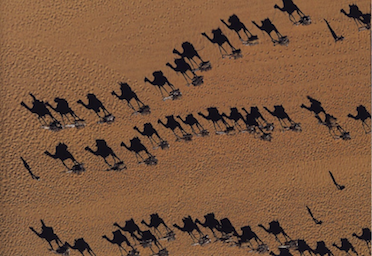
\includegraphics[width=8cm]{camels.png} \\
Figure 21: Common fate provides visual cues for the segmentation problem; source: Arthus-Bertrand (via F. Durand)
\end{center}

We can also illustrate common fate with this optical illusion. This illusion, called the Müller-Lyer illusion, tricks us into thinking the bottom line segment is longer than the top line segment, even though they are actually the same length (disregarding the four mini-tails).

\begin{center}
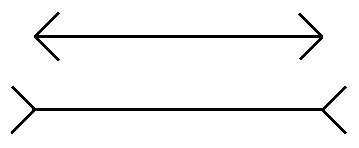
\includegraphics[width=8cm]{muller.jpg} \\
Figure 22: Common fate results in an optical illusion; source: Simon Barthelme
\end{center}

Another way we can group objects is by proximity. With proximity, we group objects with what they appear to be close to. For instance, in this image, we might group the three people in the foreground together.
\begin{center}
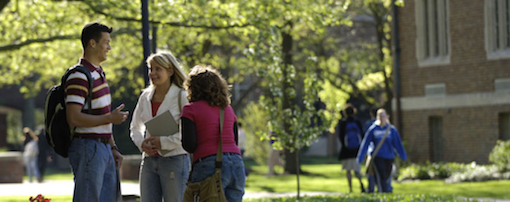
\includegraphics[width=8cm]{people.png} \\
Figure 23: Proximity can aid the image segmentation; source: Kristen Grauman
\end{center}


% References
\small
\bibliographystyle{plain}
\bibliography{bibliography}
\end{document} 